\section{Background Information, Related Work and Research}
In the following chapter, we further explore the motivation for undertaking the project,
analyse the current state of the project domain and outline the research that forms the basis for the rest of the report.

\subsection{The Problem}
As previously mentioned, the goal of this project is to automate the feature selection process for a website fingerprinting attack.
By this we mean that given a specific trace, our model should be able to produce a fixed-length vector that is a close representation of the respective trace.
However, before we delve into the details of the attack, we first need to gain a greater understanding of some concepts such as
onion routing, website fingerprinting in general and deep learning.

\subsubsection{Onion Routing}
To preserve privacy, we do not only need to obscure the content of a webpage but also hide who is taking to whom \cite{goldschlag1999onion}.
Tor achieves both of these by making use of a technique, called \textit{onion routing}, which is a very simple protocol that can be divided up into three phases:
connection setup, data movement and connection tear-down \cite{goldschlag1999onion}. We show how it works by taking a simple example of Alice trying to communicate with Bob.

\begin{enumerate}
  \item \textbf{Connection Setup:}
    \begin{itemize}
      \item Alice's Tor client obtains a list of Tor nodes from a directory server.
      \item Then Alice picks three random Tor nodes and labels them \textit{one, two} and \textit{three}.
      \item Alice communicates with the first node and shares a symmetric key.
      \item Next, Alice sends messages to the first node, which are then forwarded to the second node to share another symmetric key to the second node.
      \item Finally, Alice continues sending messages to the first node, which are forwarded to the second and finally to the third node to share the final symmetric key.
        What is important here is that we use a secure key-sharing algorithm such that only Alice and the respective node know the keys.
        Additionally, since all of the traffic is forwarded from the first node, the second and the third nodes do not know the identity of Alice.
    \end{itemize}

    \begin{figure}[h]
      \centering
      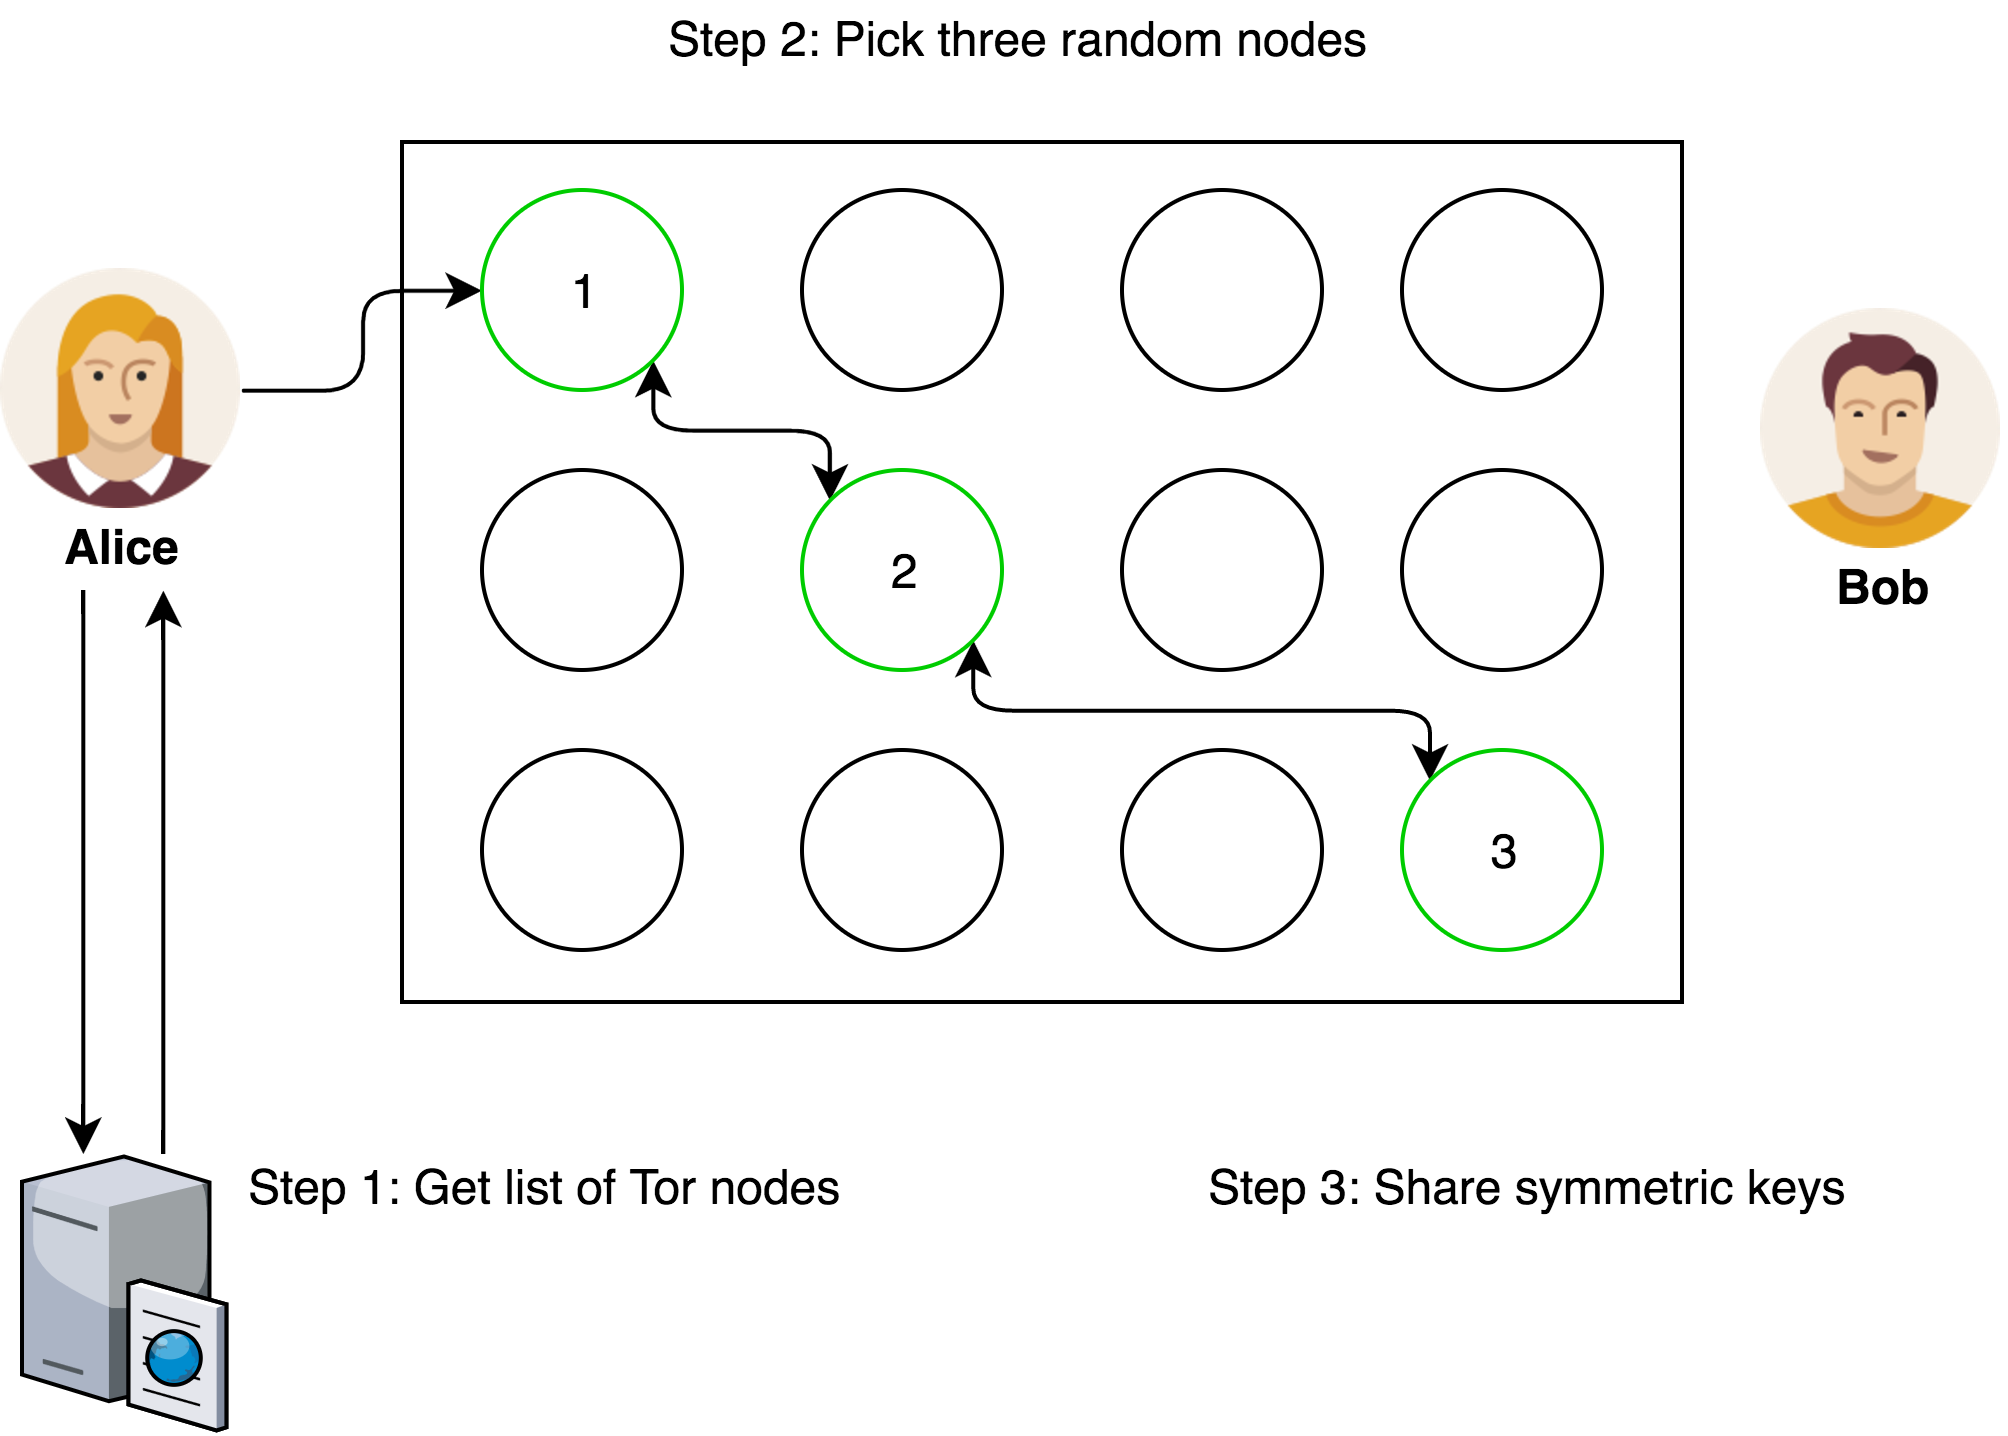
\includegraphics[width=0.75\textwidth]{tor_setup}
      \caption{An example of a connection setup for the onion routing protocol.}
      \label{fig:tor_setup}
    \end{figure}

  \item \textbf{Data Movement:}
    \begin{itemize}
      \item Before Alice can send any data, it first needs to encrypt it in different layers. By this we mean that first it encrypts the data \textit{(with Bob's address)}
        using the shared key from the third node. Next, it encrypts that data again \textit{(with the address of the third node)} using the key from the second node.
        Finally, as expected, it encrypts the data a final time \textit{(with the address of the second node)} using the shared key from the first node.

      \item Now Alice is ready to send the data to the first node.
      \item Once the first node received the data, it decrypts it using the shared key. This reveals the address to the second node.
        The key is here that the first node cannot see the data nor where it is going, since that is still encrypted.

      \item Next, the first node forwards the data that it just unencrypted to the second node. Again, this node decrypts the data, revealing the address to the third node
        but now it doesn't know what the data is, where the final destination is or where it originally came from.

      \item Lastly, the second node forwards the data to the third node. After encryption, this final node can see the data and where it is going but it does not know where it came from.
        So it forwards the data to Bob and not a single party should be able to know the data, the final destination and where it originally came from except for Alice and Bob.
    \end{itemize}

    Now we know why the protocol is called onion routing because it encrypts the data in multiple layers and at every node, one of the layers of the onion is peeled off \cite{tor_project2}.
    The key is that none of the nodes know the complete path that has been taken.

    \begin{figure}[h]
      \centering
      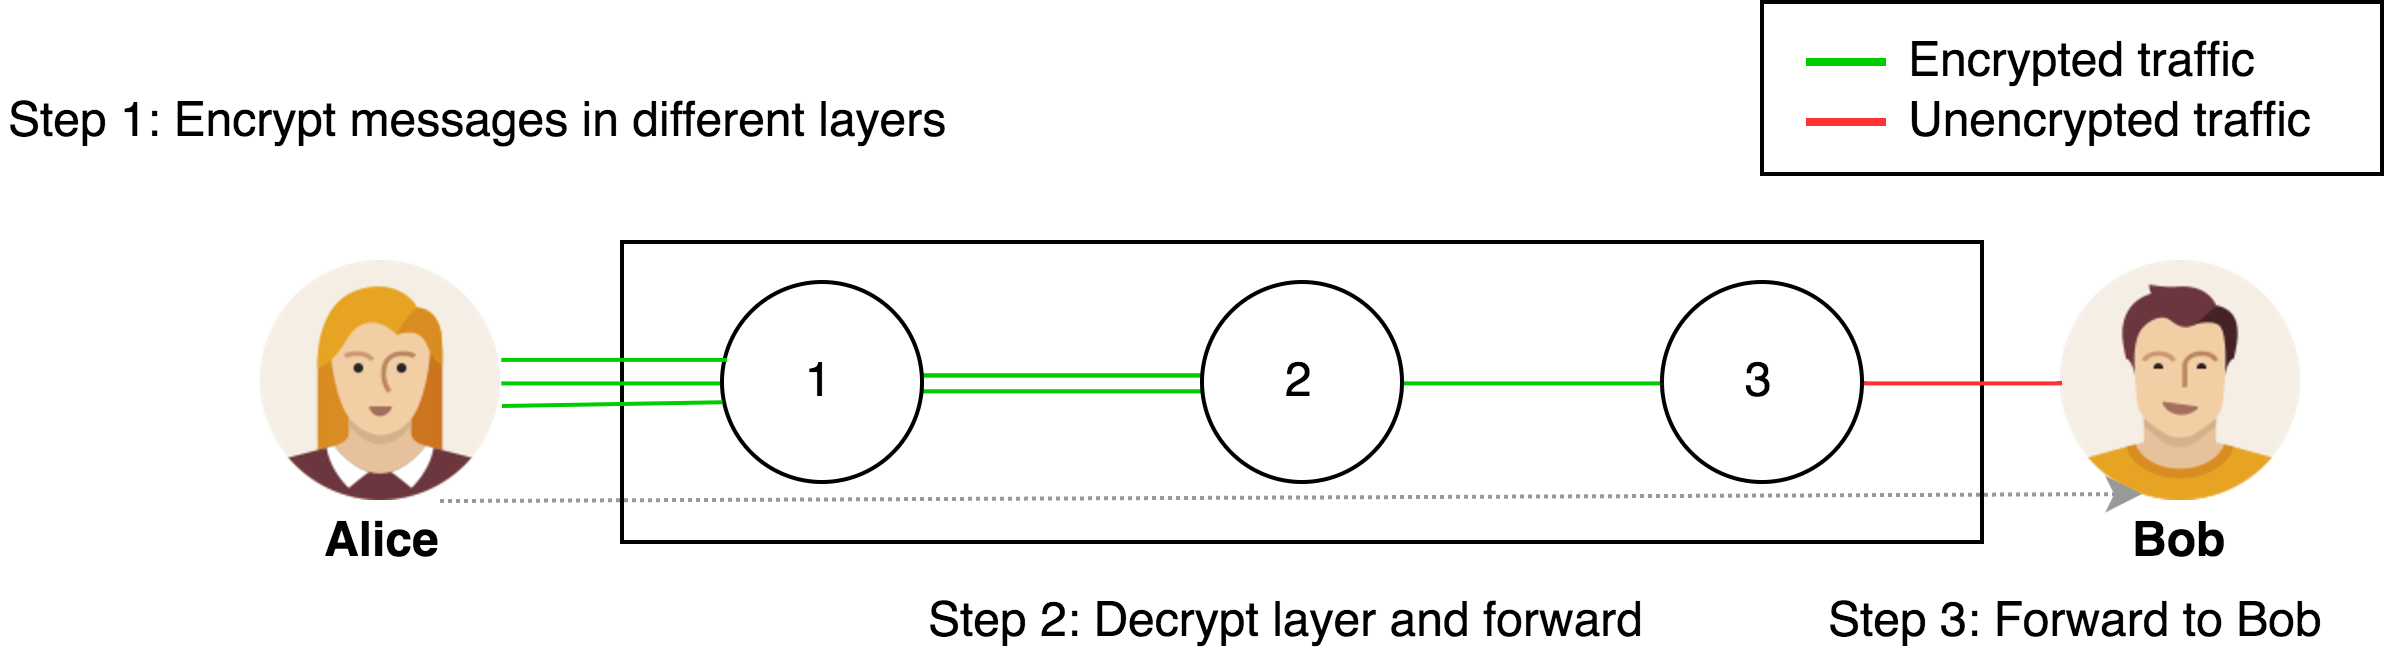
\includegraphics[width=0.75\textwidth]{tor_message_sending}
      \caption{Sending a message with the onion routing protocol.}
      \label{fig:tor_message_sending}
    \end{figure}

  \item \textbf{Connection Tear-down:} This can be initiated by any of the nodes or the client and the process is very straightforward.
    Either the client sends a request for a tear-down to the first node to remove any data on the connection (including the shared key), which is then forwarded to the other nodes.
    Or one of the nodes sends a tear-down message to both the previous node and the next node, which are then forwarded in both directions \cite{goldschlag1999onion}.

\end{enumerate}

Tor generally uses the same circuit for connections that happen within around 10 minutes after creating a circuit.
Later requests, however, are given a new circuit \cite{tor_project, tor_project2}.

\subsection{Related Work}

\subsubsection{Website Fingerprinting}

\subsubsection{Defenses}

\subsubsection{Critical Analysis}

\subsection{Deep Learning}

\subsection{Automatic Feature Selection}

\subsubsection{Stacked Authoencoder}

\subsubsection{Sequence-to-Sequence Model}

\subsection{Software Libraries}
